\section{Intelligence Artificielle et Industrie 4.0}\label{chap3:ia_industrie40}

\subsection{Qu'est-ce que l'Intelligence Artificielle?}

L'Intelligence Artificielle (IA) représente l'un des domaines les plus transformateurs de l'informatique moderne, visant à créer des systèmes capables d'effectuer des tâches qui nécessitent traditionnellement l'intelligence humaine. Selon \cite{russell2010artificial}, l'IA peut être définie comme \textit{"l'étude et la conception d'agents intelligents capables de percevoir leur environnement et de prendre des actions qui maximisent leurs chances de succès"}.

\subsubsection{Définitions et concepts fondamentaux}

L'Intelligence Artificielle englobe plusieurs paradigmes et approches complémentaires :

\begin{itemize}
    \item \textbf{Intelligence Artificielle symbolique} : Approche basée sur la manipulation de symboles et de règles logiques, dominante dans les années 1950-1980
    \item \textbf{Machine Learning (Apprentissage Automatique)} : Capacité des systèmes à apprendre à partir de données sans être explicitement programmés \cite{mitchell1997machine}
    \item \textbf{Deep Learning (Apprentissage Profond)} : Sous-domaine du ML utilisant des réseaux de neurones artificiels profonds pour modéliser des abstractions complexes
    \item \textbf{IA symbolique vs connexionniste} : Opposition historique entre approches basées sur la logique et celles basées sur les réseaux de neurones
\end{itemize}

\subsubsection{Évolution historique de l'IA}

L'histoire de l'Intelligence Artificielle peut être divisée en plusieurs périodes clés :

\begin{table}[H]
\centering
\caption{Évolution historique de l'Intelligence Artificielle}
\begin{tabular}{|l|l|p{8cm}|}
\hline
\textbf{Période} & \textbf{Nom} & \textbf{Caractéristiques principales} \\
\hline
1950-1956 & Genèse & Test de Turing (1950), Conférence de Dartmouth (1956), naissance officielle de l'IA \\
\hline
1956-1974 & Âge d'or & Optimisme, premiers programmes (Logic Theorist, ELIZA), systèmes experts \\
\hline
1974-1980 & Premier hiver & Désillusion, limitations computationnelles, réduction des financements \\
\hline
1980-1987 & Renaissance & Systèmes experts commerciaux, réseaux de neurones (backpropagation) \\
\hline
1987-1993 & Second hiver & Échec des systèmes experts, limitations des approches symboliques \\
\hline
1993-2011 & Maturité & Approches probabilistes, SVM, Random Forests, applications pratiques \\
\hline
2012-présent & Révolution Deep Learning & AlexNet (2012), explosion des données, GPU, succès spectaculaires \\
\hline
\end{tabular}
\label{tab:ia_history}
\end{table}

La période actuelle (depuis 2012) est marquée par des avancées spectaculaires grâce à la convergence de trois facteurs : (1) la disponibilité massive de données (Big Data), (2) la puissance de calcul accrue (GPU, TPU), et (3) les innovations algorithmiques (architectures de réseaux de neurones profonds).

\subsubsection{Types d'Intelligence Artificielle}

On distingue traditionnellement plusieurs niveaux d'IA selon leurs capacités :

\textbf{1. IA Faible (Narrow AI ou Weak AI)}

L'IA faible désigne des systèmes conçus pour accomplir des tâches spécifiques dans un domaine limité. C'est le type d'IA actuellement déployé dans l'industrie.

\textbf{Caractéristiques :}
\begin{itemize}
    \item Spécialisée dans une tâche précise (reconnaissance d'images, traduction, jeu d'échecs)
    \item Performance souvent supérieure à l'humain dans son domaine
    \item Incapable de généraliser à d'autres domaines
    \item Exemples : AlphaGo, systèmes de recommandation, assistants vocaux
\end{itemize}

\textbf{2. IA Forte (General AI ou Strong AI)}

L'IA forte représente un système hypothétique possédant une intelligence comparable à celle de l'humain, capable de raisonner, planifier et apprendre dans n'importe quel domaine.

\textbf{Caractéristiques :}
\begin{itemize}
    \item Capacité de généralisation universelle
    \item Conscience et compréhension du monde
    \item Apprentissage autonome multi-domaines
    \item Statut : Objectif de recherche à long terme, non atteint actuellement
\end{itemize}

\textbf{3. Super-Intelligence Artificielle}

Concept théorique d'une IA dépassant largement les capacités cognitives humaines dans tous les domaines. Sujet de débats éthiques et philosophiques \cite{bostrom2014superintelligence}.

\subsubsection{Paradigmes d'apprentissage en Machine Learning}

Le Machine Learning, cœur de l'IA moderne, se décline en plusieurs paradigmes d'apprentissage :

\begin{figure}[H]
\centering
\begin{tikzpicture}[
    node distance=2cm,
    box/.style={rectangle, draw, fill=blue!15, text width=3.5cm, text centered, rounded corners, minimum height=1.2cm, font=\small},
    arrow/.style={->, >=stealth, thick}
]

\node[box, fill=green!20] (ml) at (0,0) {\textbf{Machine Learning}};

\node[box] (supervised) at (-4,-2.5) {\textbf{Apprentissage\\Supervisé}};
\node[box] (unsupervised) at (0,-2.5) {\textbf{Apprentissage\\Non-Supervisé}};
\node[box] (reinforcement) at (4,-2.5) {\textbf{Apprentissage\\par Renforcement}};

\draw[arrow] (ml) -- (supervised);
\draw[arrow] (ml) -- (unsupervised);
\draw[arrow] (ml) -- (reinforcement);

\node[below=0.3cm of supervised, font=\footnotesize, text width=3.5cm, align=center] {
    Données étiquetées\\
    Classification, Régression
};

\node[below=0.3cm of unsupervised, font=\footnotesize, text width=3.5cm, align=center] {
    Données non étiquetées\\
    Clustering, Réduction
};

\node[below=0.3cm of reinforcement, font=\footnotesize, text width=3.5cm, align=center] {
    Récompenses/Pénalités\\
    Jeux, Robotique
};

\end{tikzpicture}
\caption{Paradigmes d'apprentissage en Machine Learning}
\label{fig:ml_paradigms}
\end{figure}

\textbf{Apprentissage Supervisé :}
\begin{itemize}
    \item Données d'entraînement étiquetées (paires entrée-sortie)
    \item Objectif : Apprendre une fonction de mapping $f: X \rightarrow Y$
    \item Applications : Classification (spam/non-spam), Régression (prédiction de prix)
    \item Algorithmes : Régression linéaire, SVM, Random Forest, XGBoost, Réseaux de neurones
\end{itemize}

\textbf{Apprentissage Non-Supervisé :}
\begin{itemize}
    \item Données sans étiquettes
    \item Objectif : Découvrir des structures cachées dans les données
    \item Applications : Segmentation clients, Détection d'anomalies, Réduction de dimensionnalité
    \item Algorithmes : K-means, DBSCAN, PCA, Autoencoders
\end{itemize}

\textbf{Apprentissage par Renforcement :}
\begin{itemize}
    \item Agent apprenant par interaction avec un environnement
    \item Objectif : Maximiser une récompense cumulative
    \item Applications : Jeux (AlphaGo), Robotique, Véhicules autonomes
    \item Algorithmes : Q-Learning, Deep Q-Networks (DQN), Policy Gradients
\end{itemize}

\subsubsection{Applications actuelles de l'IA}

L'IA est aujourd'hui déployée dans de nombreux secteurs avec des impacts mesurables :

\begin{table}[H]
\centering
\caption{Applications de l'IA par secteur}
\begin{tabular}{|l|p{5cm}|p{5cm}|}
\hline
\textbf{Secteur} & \textbf{Applications} & \textbf{Impact} \\
\hline
Santé & Diagnostic médical, découverte de médicaments, imagerie médicale & Précision diagnostique +20\%, réduction temps R\&D \\
\hline
Finance & Détection de fraude, trading algorithmique, scoring crédit & Réduction fraude -40\%, optimisation portefeuilles \\
\hline
Transport & Véhicules autonomes, optimisation logistique, maintenance prédictive & Réduction accidents -90\%, économies carburant -15\% \\
\hline
Retail & Recommandations personnalisées, gestion stocks, pricing dynamique & Augmentation ventes +30\%, réduction ruptures -25\% \\
\hline
Industrie & Contrôle qualité, maintenance prédictive, optimisation production & Réduction défauts -50\%, disponibilité +20\% \\
\hline
\end{tabular}
\label{tab:ia_applications}
\end{table}

Dans le contexte de ce projet, nous nous concentrons sur l'\textbf{apprentissage supervisé} pour la prédiction des temps de matelassage et sur l'\textbf{optimisation combinatoire} pour l'ordonnancement des tables de coupe.


\subsection{L'Industrie 4.0 et la Transformation Digitale}

\subsubsection{Définition de l'Industrie 4.0}

L'Industrie 4.0, également appelée \textit{Quatrième Révolution Industrielle}, désigne la transformation digitale profonde des processus de fabrication et de production industrielle. Le terme a été introduit en 2011 lors du salon de Hanovre en Allemagne \cite{kagermann2013recommendations} et représente l'intégration des technologies numériques avancées dans l'ensemble de la chaîne de valeur industrielle.

\textbf{Définition formelle :} L'Industrie 4.0 est caractérisée par la convergence des technologies physiques, numériques et biologiques, créant des systèmes cyber-physiques (CPS) interconnectés capables de prendre des décisions autonomes et d'optimiser les processus de production en temps réel \cite{schwab2017fourth}.

\subsubsection{Les quatre révolutions industrielles}

L'histoire industrielle peut être divisée en quatre révolutions majeures, chacune marquée par une innovation technologique disruptive :

\begin{figure}[H]
\centering
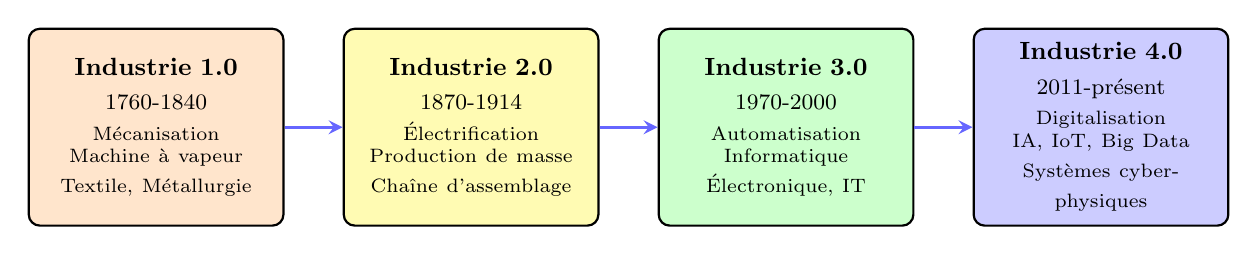
\begin{tikzpicture}[
    node distance=1.5cm,
    revolution/.style={rectangle, draw, thick, text width=3cm, text centered, rounded corners, minimum height=2.5cm, font=\small},
    arrow/.style={->, >=stealth, very thick, blue!60}
]

\node[revolution, fill=orange!20] (rev1) at (0,0) {
    \textbf{Industrie 1.0}\\[3pt]
    \footnotesize 1760-1840\\[3pt]
    \scriptsize Mécanisation\\
    Machine à vapeur\\
    Textile, Métallurgie
};

\node[revolution, fill=yellow!30] (rev2) at (4,0) {
    \textbf{Industrie 2.0}\\[3pt]
    \footnotesize 1870-1914\\[3pt]
    \scriptsize Électrification\\
    Production de masse\\
    Chaîne d'assemblage
};

\node[revolution, fill=green!20] (rev3) at (8,0) {
    \textbf{Industrie 3.0}\\[3pt]
    \footnotesize 1970-2000\\[3pt]
    \scriptsize Automatisation\\
    Informatique\\
    Électronique, IT
};

\node[revolution, fill=blue!20] (rev4) at (12,0) {
    \textbf{Industrie 4.0}\\[3pt]
    \footnotesize 2011-présent\\[3pt]
    \scriptsize Digitalisation\\
    IA, IoT, Big Data\\
    Systèmes cyber-physiques
};

\draw[arrow] (rev1) -- (rev2);
\draw[arrow] (rev2) -- (rev3);
\draw[arrow] (rev3) -- (rev4);

\end{tikzpicture}
\caption{Les quatre révolutions industrielles}
\label{fig:industrial_revolutions}
\end{figure}

\textbf{Industrie 1.0 (1760-1840) - Mécanisation}
\begin{itemize}
    \item \textbf{Innovation clé} : Machine à vapeur (James Watt, 1769)
    \item \textbf{Impact} : Remplacement de la force humaine/animale par la force mécanique
    \item \textbf{Secteurs} : Textile, métallurgie, transport ferroviaire
    \item \textbf{Gains} : Productivité multipliée par 10-20
\end{itemize}

\textbf{Industrie 2.0 (1870-1914) - Électrification et Production de Masse}
\begin{itemize}
    \item \textbf{Innovation clé} : Électricité, moteur à combustion interne
    \item \textbf{Impact} : Production de masse, standardisation, division du travail
    \item \textbf{Symbole} : Chaîne d'assemblage de Ford (1913)
    \item \textbf{Gains} : Réduction coûts de 60-70\%, démocratisation des produits
\end{itemize}

\textbf{Industrie 3.0 (1970-2000) - Automatisation et Informatisation}
\begin{itemize}
    \item \textbf{Innovation clé} : Ordinateurs, automates programmables (PLC), robots
    \item \textbf{Impact} : Automatisation des tâches répétitives, contrôle numérique
    \item \textbf{Technologies} : ERP, MES, SCADA, CAO/FAO
    \item \textbf{Gains} : Flexibilité +40\%, qualité +30\%, réduction main d'œuvre
\end{itemize}

\textbf{Industrie 4.0 (2011-présent) - Digitalisation et Intelligence}
\begin{itemize}
    \item \textbf{Innovation clé} : IA, IoT, Big Data, Cloud, Cyber-sécurité
    \item \textbf{Impact} : Systèmes autonomes, décisions en temps réel, personnalisation de masse
    \item \textbf{Paradigme} : Usine intelligente (Smart Factory), jumeau numérique (Digital Twin)
    \item \textbf{Gains attendus} : Productivité +30\%, flexibilité +50\%, time-to-market -40\%
\end{itemize}

\subsubsection{Les piliers technologiques de l'Industrie 4.0}

L'Industrie 4.0 repose sur neuf piliers technologiques interconnectés \cite{rüßmann2015industry} :

\begin{figure}[H]
\centering
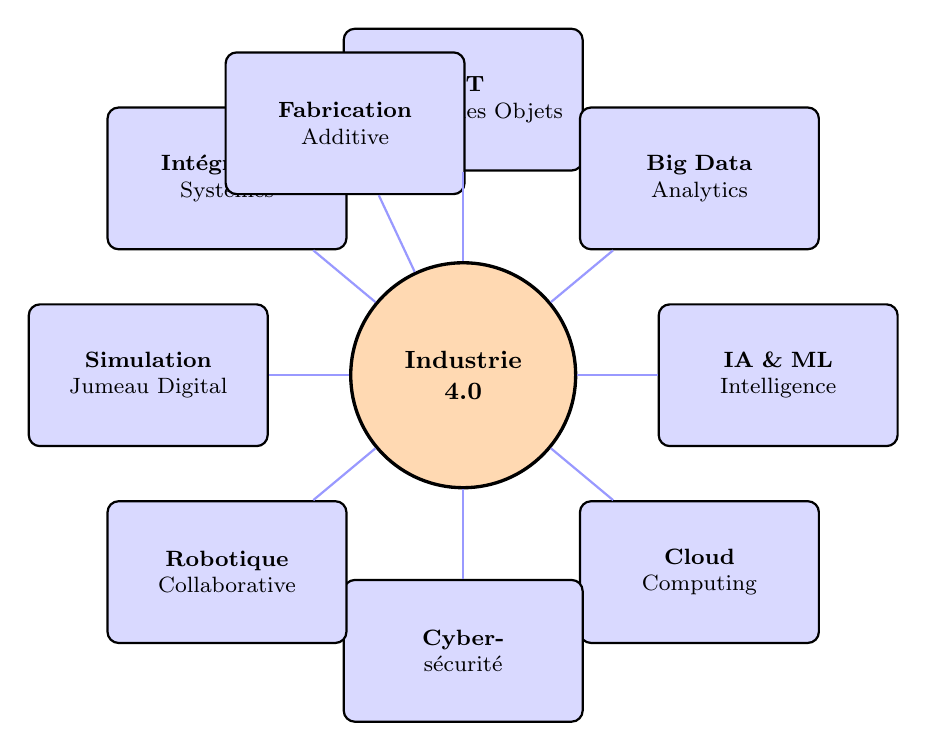
\begin{tikzpicture}[
    node distance=0.3cm,
    pillar/.style={rectangle, draw, thick, fill=blue!15, text width=2.8cm, text centered, rounded corners, minimum height=1.8cm, font=\footnotesize},
    center/.style={circle, draw, very thick, fill=orange!30, text width=2.5cm, text centered, font=\small\bfseries}
]

% Centre
\node[center] (center) at (0,0) {Industrie\\4.0};

% Piliers autour (disposition circulaire)
\node[pillar] (iot) at (0,3.5) {\textbf{IoT}\\Internet des Objets};
\node[pillar] (bigdata) at (3,2.5) {\textbf{Big Data}\\Analytics};
\node[pillar] (ai) at (4,0) {\textbf{IA \& ML}\\Intelligence};
\node[pillar] (cloud) at (3,-2.5) {\textbf{Cloud}\\Computing};
\node[pillar] (cyber) at (0,-3.5) {\textbf{Cyber-}\\sécurité};
\node[pillar] (robot) at (-3,-2.5) {\textbf{Robotique}\\Collaborative};
\node[pillar] (simulation) at (-4,0) {\textbf{Simulation}\\Jumeau Digital};
\node[pillar] (integration) at (-3,2.5) {\textbf{Intégration}\\Systèmes};
\node[pillar] (additive) at (-1.5,3.2) {\textbf{Fabrication}\\Additive};

% Connexions
\foreach \pillar in {iot, bigdata, ai, cloud, cyber, robot, simulation, integration, additive}
    \draw[thick, blue!40] (center) -- (\pillar);

\end{tikzpicture}
\caption{Les neuf piliers technologiques de l'Industrie 4.0}
\label{fig:industry40_pillars}
\end{figure}

\textbf{1. Internet des Objets (IoT - Internet of Things)}

Réseau de capteurs et d'actionneurs connectés collectant et échangeant des données en temps réel.

\begin{itemize}
    \item \textbf{Technologies} : Capteurs RFID, NFC, Bluetooth, LoRa, 5G
    \item \textbf{Applications} : Suivi des actifs, monitoring machines, traçabilité produits
    \item \textbf{Impact} : Visibilité temps réel, maintenance prédictive, optimisation énergétique
    \item \textbf{Chiffres} : 75 milliards d'objets connectés prévus en 2025 (IDC)
\end{itemize}

\textbf{2. Big Data et Analytics}

Capacité à collecter, stocker et analyser des volumes massifs de données hétérogènes.

\begin{itemize}
    \item \textbf{Caractéristiques} : Volume (pétaoctets), Vélocité (temps réel), Variété (structuré/non-structuré)
    \item \textbf{Technologies} : Hadoop, Spark, NoSQL, Data Lakes
    \item \textbf{Applications} : Analyse prédictive, détection d'anomalies, optimisation processus
    \item \textbf{Impact} : Décisions data-driven, amélioration continue, innovation produits
\end{itemize}

\textbf{3. Intelligence Artificielle et Machine Learning}

Systèmes capables d'apprendre, de raisonner et de prendre des décisions autonomes.

\begin{itemize}
    \item \textbf{Techniques} : Apprentissage supervisé, non-supervisé, par renforcement, Deep Learning
    \item \textbf{Applications} : Prédiction demande, contrôle qualité visuel, optimisation planning
    \item \textbf{Impact} : Automatisation décisions complexes, personnalisation, efficacité +25-40\%
    \item \textbf{Investissements} : 500 milliards USD prévus en 2024 (IDC)
\end{itemize}

\textbf{4. Cloud Computing}

Infrastructure informatique distribuée accessible à la demande via Internet.

\begin{itemize}
    \item \textbf{Modèles} : IaaS, PaaS, SaaS, Edge Computing
    \item \textbf{Avantages} : Scalabilité, flexibilité, réduction coûts IT, accessibilité
    \item \textbf{Applications} : ERP cloud, MES cloud, collaboration, backup
    \item \textbf{Adoption} : 94\% des entreprises utilisent le cloud (Flexera 2023)
\end{itemize}

\textbf{5. Cyber-sécurité}

Protection des systèmes industriels contre les cyberattaques et les intrusions.

\begin{itemize}
    \item \textbf{Enjeux} : Interconnexion accrue = surface d'attaque élargie
    \item \textbf{Technologies} : Firewalls industriels, détection d'intrusion, chiffrement
    \item \textbf{Standards} : IEC 62443, ISO 27001, NIST Cybersecurity Framework
    \item \textbf{Coût} : Cyberattaques coûtent 6 trillions USD/an globalement (Cybersecurity Ventures)
\end{itemize}

\textbf{6. Robotique Collaborative (Cobots)}

Robots conçus pour travailler en collaboration directe avec les humains.

\begin{itemize}
    \item \textbf{Caractéristiques} : Sécurité intrinsèque, facilité de programmation, flexibilité
    \item \textbf{Applications} : Assemblage, pick-and-place, contrôle qualité, emballage
    \item \textbf{Impact} : Productivité +30\%, ergonomie améliorée, réduction TMS
    \item \textbf{Marché} : Croissance 40\% CAGR 2020-2027 (MarketsandMarkets)
\end{itemize}

\textbf{7. Simulation et Jumeau Numérique (Digital Twin)}

Réplique virtuelle d'un système physique permettant simulation et optimisation.

\begin{itemize}
    \item \textbf{Concept} : Modèle numérique synchronisé avec le système réel via IoT
    \item \textbf{Applications} : Test de scénarios, optimisation paramètres, formation, maintenance
    \item \textbf{Impact} : Réduction time-to-market -50\%, coûts R\&D -30\%, qualité +25\%
    \item \textbf{Adoption} : 75\% des grandes entreprises industrielles en 2025 (Gartner)
\end{itemize}

\textbf{8. Intégration Horizontale et Verticale}

Interconnexion des systèmes à tous les niveaux de l'entreprise et de la chaîne de valeur.

\begin{itemize}
    \item \textbf{Verticale} : ERP $\leftrightarrow$ MES $\leftrightarrow$ SCADA $\leftrightarrow$ Capteurs (pyramide CIM)
    \item \textbf{Horizontale} : Intégration fournisseurs-production-clients (Supply Chain)
    \item \textbf{Technologies} : API, middleware, bus de données, standards (OPC UA)
    \item \textbf{Impact} : Visibilité end-to-end, agilité, réduction silos
\end{itemize}

\textbf{9. Fabrication Additive (Impression 3D)}

Technologies de fabrication par ajout de matière couche par couche.

\begin{itemize}
    \item \textbf{Procédés} : FDM, SLA, SLS, DMLS (métaux)
    \item \textbf{Applications} : Prototypage rapide, pièces de rechange, personnalisation
    \item \textbf{Impact} : Réduction délais -70\%, complexité géométrique, production décentralisée
    \item \textbf{Marché} : 50 milliards USD en 2028 (Wohlers Report)
\end{itemize}


\subsubsection{Bénéfices et impacts de l'Industrie 4.0}

L'adoption de l'Industrie 4.0 génère des bénéfices mesurables à plusieurs niveaux :

\begin{table}[H]
\centering
\caption{Bénéfices quantifiés de l'Industrie 4.0}
\begin{tabular}{|l|l|p{6cm}|}
\hline
\textbf{Dimension} & \textbf{Amélioration} & \textbf{Leviers} \\
\hline
Productivité & +20-30\% & Automatisation, optimisation temps réel, réduction gaspillages \\
\hline
Qualité & +25-35\% & Contrôle qualité automatisé, traçabilité, maintenance prédictive \\
\hline
Flexibilité & +40-50\% & Reconfiguration rapide, personnalisation de masse, agilité \\
\hline
Time-to-Market & -30-50\% & Simulation, prototypage rapide, collaboration digitale \\
\hline
Coûts opérationnels & -15-25\% & Efficacité énergétique, réduction stocks, optimisation ressources \\
\hline
Disponibilité équipements & +10-20\% & Maintenance prédictive, monitoring continu, réduction pannes \\
\hline
Satisfaction client & +20-30\% & Personnalisation, qualité, délais réduits, traçabilité \\
\hline
\end{tabular}
\label{tab:industry40_benefits}
\end{table}

\textbf{Impact économique global :}

Selon le World Economic Forum \cite{wef2020future}, l'Industrie 4.0 pourrait générer :
\begin{itemize}
    \item \textbf{3,7 trillions USD} de valeur ajoutée d'ici 2025
    \item \textbf{100 millions} de nouveaux emplois créés (transformation des compétences)
    \item \textbf{Réduction de 10-20\%} de l'empreinte carbone industrielle
    \item \textbf{Augmentation de 15-25\%} du PIB manufacturier dans les pays adopteurs
\end{itemize}

\subsubsection{Défis et barrières à l'adoption}

Malgré ses bénéfices, l'Industrie 4.0 fait face à plusieurs défis majeurs :

\textbf{1. Défis technologiques}
\begin{itemize}
    \item Complexité d'intégration des systèmes legacy
    \item Interopérabilité entre technologies hétérogènes
    \item Gestion de la qualité et de la sécurité des données
    \item Infrastructure réseau insuffisante (bande passante, latence)
\end{itemize}

\textbf{2. Défis organisationnels}
\begin{itemize}
    \item Résistance au changement culturel
    \item Manque de compétences digitales (data scientists, ingénieurs IA)
    \item Transformation des processus et des rôles
    \item Collaboration inter-départements nécessaire
\end{itemize}

\textbf{3. Défis financiers}
\begin{itemize}
    \item Investissements initiaux élevés (ROI à moyen terme)
    \item Difficulté à quantifier les bénéfices intangibles
    \item Coûts de formation et de conduite du changement
    \item Risque d'obsolescence technologique rapide
\end{itemize}

\textbf{4. Défis stratégiques}
\begin{itemize}
    \item Absence de vision et de stratégie claire
    \item Manque de soutien du top management
    \item Difficulté à prioriser les initiatives
    \item Écosystème de partenaires technologiques complexe
\end{itemize}

\subsection{Le Rôle de l'Intelligence Artificielle dans l'Industrie 4.0}

\subsubsection{L'IA comme catalyseur de l'Industrie 4.0}

L'Intelligence Artificielle occupe une position centrale dans l'Industrie 4.0, agissant comme le \textit{"cerveau"} des systèmes cyber-physiques. Alors que l'IoT fournit les \textit{"sens"} (capteurs) et le Cloud l'infrastructure de stockage et de calcul, l'IA apporte la capacité de \textit{comprendre, apprendre et décider} de manière autonome.

\begin{figure}[H]
\centering
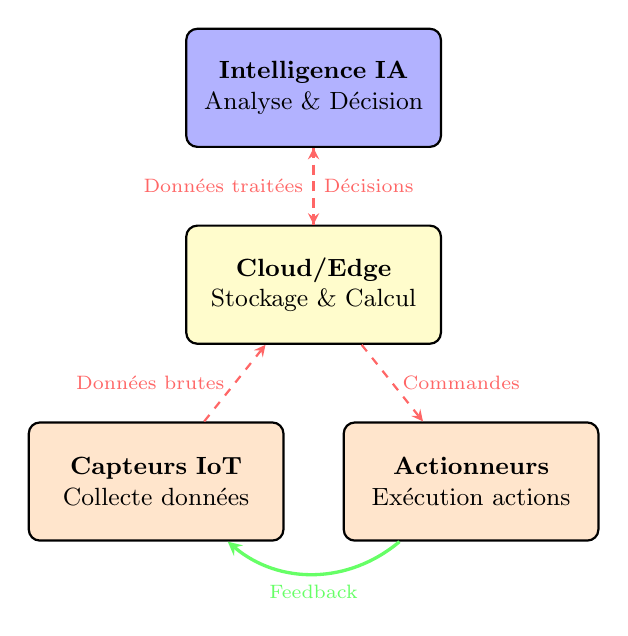
\begin{tikzpicture}[
    node distance=1.8cm,
    component/.style={rectangle, draw, thick, text width=3cm, text centered, rounded corners, minimum height=1.5cm, font=\small},
    arrow/.style={->, >=stealth, very thick},
    data/.style={->, >=stealth, thick, dashed, red!60}
]

% Couche physique
\node[component, fill=orange!20] (sensors) at (0,0) {\textbf{Capteurs IoT}\\Collecte données};
\node[component, fill=orange!20] (actuators) at (4,0) {\textbf{Actionneurs}\\Exécution actions};

% Couche données
\node[component, fill=yellow!20] (cloud) at (2,2.5) {\textbf{Cloud/Edge}\\Stockage \& Calcul};

% Couche intelligence
\node[component, fill=blue!30] (ai) at (2,5) {\textbf{Intelligence IA}\\Analyse \& Décision};

% Flux de données
\draw[data] (sensors) -- node[left, font=\scriptsize] {Données brutes} (cloud);
\draw[data] (cloud) -- node[left, font=\scriptsize] {Données traitées} (ai);
\draw[data] (ai) -- node[right, font=\scriptsize] {Décisions} (cloud);
\draw[data] (cloud) -- node[right, font=\scriptsize] {Commandes} (actuators);

% Boucle de feedback
\draw[arrow, green!60, bend left=40] (actuators) to node[below, font=\scriptsize] {Feedback} (sensors);

\end{tikzpicture}
\caption{Architecture de l'IA dans l'Industrie 4.0}
\label{fig:ai_industry40_architecture}
\end{figure}

\subsubsection{Domaines d'application de l'IA dans l'industrie}

L'IA transforme l'ensemble de la chaîne de valeur industrielle à travers six domaines principaux :

\textbf{1. Optimisation de la Production et Planification}

L'IA permet d'optimiser les processus de production en temps réel et d'améliorer la planification.

\textbf{Applications :}
\begin{itemize}
    \item \textbf{Ordonnancement intelligent} : Optimisation de l'allocation des ressources (machines, opérateurs, matières)
    \item \textbf{Prédiction de la demande} : Anticipation des besoins clients avec précision accrue
    \item \textbf{Optimisation énergétique} : Réduction de la consommation énergétique de 10-20\%
    \item \textbf{Gestion des stocks} : Minimisation des stocks tout en évitant les ruptures
\end{itemize}

\textbf{Techniques IA utilisées :}
\begin{itemize}
    \item Machine Learning supervisé (régression, séries temporelles)
    \item Optimisation combinatoire (programmation linéaire, contraintes)
    \item Apprentissage par renforcement (décisions séquentielles)
\end{itemize}

\textbf{Gains mesurés :}
\begin{itemize}
    \item Productivité : +15-25\%
    \item Utilisation des équipements : +10-20\%
    \item Réduction des coûts : -10-15\%
    \item Time-to-market : -20-30\%
\end{itemize}

\textbf{2. Maintenance Prédictive et Prescriptive}

Anticipation des pannes et recommandation d'actions de maintenance optimales.

\textbf{Applications :}
\begin{itemize}
    \item \textbf{Prédiction de pannes} : Détection précoce des anomalies avant défaillance
    \item \textbf{Estimation de durée de vie résiduelle (RUL)} : Planification maintenance optimale
    \item \textbf{Maintenance prescriptive} : Recommandation d'actions correctives spécifiques
    \item \textbf{Optimisation des pièces de rechange} : Gestion intelligente des stocks critiques
\end{itemize}

\textbf{Techniques IA utilisées :}
\begin{itemize}
    \item Détection d'anomalies (Isolation Forest, Autoencoders)
    \item Prédiction de séries temporelles (LSTM, Prophet)
    \item Classification multi-classes (types de pannes)
\end{itemize}

\textbf{Gains mesurés :}
\begin{itemize}
    \item Réduction pannes imprévues : -30-50\%
    \item Disponibilité équipements : +10-20\%
    \item Coûts de maintenance : -20-40\%
    \item Durée de vie équipements : +20-30\%
\end{itemize}

\textbf{3. Contrôle Qualité Automatisé}

Inspection automatique et détection de défauts par vision artificielle.

\textbf{Applications :}
\begin{itemize}
    \item \textbf{Inspection visuelle} : Détection de défauts de surface, fissures, rayures
    \item \textbf{Classification de défauts} : Catégorisation automatique des non-conformités
    \item \textbf{Prédiction de qualité} : Anticipation de la qualité finale dès les premières étapes
    \item \textbf{Analyse de causes racines} : Identification des facteurs influençant la qualité
\end{itemize}

\textbf{Techniques IA utilisées :}
\begin{itemize}
    \item Deep Learning (CNN : Convolutional Neural Networks)
    \item Segmentation d'images (U-Net, Mask R-CNN)
    \item Transfer Learning (modèles pré-entraînés)
\end{itemize}

\textbf{Gains mesurés :}
\begin{itemize}
    \item Taux de détection : +95-99\% (vs 80-90\% humain)
    \item Vitesse d'inspection : 10-100x plus rapide
    \item Réduction défauts : -30-50\%
    \item Coûts qualité : -20-40\%
\end{itemize}

\textbf{4. Supply Chain Intelligente}

Optimisation de la chaîne d'approvisionnement de bout en bout.

\textbf{Applications :}
\begin{itemize}
    \item \textbf{Prévision de la demande} : Anticipation précise des besoins clients
    \item \textbf{Optimisation logistique} : Routage optimal, consolidation de chargements
    \item \textbf{Gestion des risques} : Détection précoce de perturbations (fournisseurs, transport)
    \item \textbf{Pricing dynamique} : Ajustement des prix en temps réel selon demande/offre
\end{itemize}

\textbf{Gains mesurés :}
\begin{itemize}
    \item Précision prévisions : +20-50\%
    \item Réduction stocks : -20-30\%
    \item Coûts logistiques : -10-20\%
    \item Niveau de service : +15-25\%
\end{itemize}

\textbf{5. Personnalisation de Masse}

Production personnalisée à grande échelle grâce à l'IA.

\textbf{Applications :}
\begin{itemize}
    \item \textbf{Configuration produits} : Recommandations personnalisées selon préférences clients
    \item \textbf{Optimisation de conception} : Génération automatique de designs optimaux
    \item \textbf{Planification flexible} : Adaptation rapide aux commandes personnalisées
    \item \textbf{Pricing personnalisé} : Tarification adaptée au profil client
\end{itemize}

\textbf{Gains mesurés :}
\begin{itemize}
    \item Satisfaction client : +25-40\%
    \item Taux de conversion : +15-30\%
    \item Marge : +10-20\%
    \item Fidélisation : +20-35\%
\end{itemize}

\textbf{6. Robotique et Automatisation Intelligente}

Robots et cobots dotés de capacités d'apprentissage et d'adaptation.

\textbf{Applications :}
\begin{itemize}
    \item \textbf{Pick-and-place intelligent} : Reconnaissance et saisie d'objets variés
    \item \textbf{Assemblage adaptatif} : Ajustement automatique aux variations de pièces
    \item \textbf{Navigation autonome} : AGV/AMR (véhicules guidés automatiquement)
    \item \textbf{Collaboration homme-robot} : Apprentissage par démonstration
\end{itemize}

\textbf{Techniques IA utilisées :}
\begin{itemize}
    \item Vision par ordinateur (détection d'objets, segmentation)
    \item Apprentissage par renforcement (navigation, manipulation)
    \item Imitation learning (apprentissage par démonstration)
\end{itemize}

\textbf{Gains mesurés :}
\begin{itemize}
    \item Productivité : +30-50\%
    \item Flexibilité : +40-60\%
    \item Qualité : +20-30\%
    \item Ergonomie : Réduction TMS -50\%
\end{itemize}


\subsubsection{Cas d'usage industriels de l'IA}

\textbf{Cas 1 : Siemens - Maintenance Prédictive}

Siemens utilise l'IA pour la maintenance prédictive de ses turbines à gaz industrielles.

\begin{itemize}
    \item \textbf{Problème} : Pannes imprévues coûteuses (1M€/jour d'arrêt)
    \item \textbf{Solution} : Modèles ML analysant 1000+ capteurs en temps réel
    \item \textbf{Résultats} : Réduction pannes -30\%, disponibilité +15\%, économies 10M€/an
\end{itemize}

\textbf{Cas 2 : BMW - Contrôle Qualité Visuel}

BMW déploie la vision artificielle pour l'inspection de carrosseries.

\begin{itemize}
    \item \textbf{Problème} : Inspection manuelle lente et subjective
    \item \textbf{Solution} : CNN détectant défauts de peinture, bosses, rayures
    \item \textbf{Résultats} : Précision 99,7\% (vs 90\% humain), vitesse 10x, coûts -40\%
\end{itemize}

\textbf{Cas 3 : Amazon - Optimisation Logistique}

Amazon utilise l'IA pour optimiser ses opérations d'entrepôt.

\begin{itemize}
    \item \textbf{Problème} : Complexité croissante (millions de SKU, délais courts)
    \item \textbf{Solution} : ML pour prévision demande, routage optimal, placement produits
    \item \textbf{Résultats} : Coûts logistiques -20\%, délais -30\%, satisfaction +25\%
\end{itemize}

\subsection{L'IA dans l'Industrie Textile}

\subsubsection{Spécificités et défis du secteur textile}

L'industrie textile présente des caractéristiques uniques qui rendent l'application de l'IA particulièrement pertinente mais aussi complexe :

\textbf{Caractéristiques du secteur :}
\begin{itemize}
    \item \textbf{Variabilité élevée} : Diversité des matières (coton, synthétique, mélanges), des produits (vêtements, linge, technique), des processus
    \item \textbf{Saisonnalité forte} : Collections saisonnières, mode éphémère, cycles courts
    \item \textbf{Personnalisation croissante} : Demande de customisation, petites séries
    \item \textbf{Pression sur les coûts} : Concurrence internationale, délocalisation
    \item \textbf{Contraintes qualité} : Exigences esthétiques et fonctionnelles élevées
    \item \textbf{Complexité de la Supply Chain} : Nombreux intervenants, délais longs
\end{itemize}

\textbf{Défis spécifiques :}
\begin{itemize}
    \item \textbf{Gestion de la variabilité} : Matières premières non homogènes, comportements imprévisibles
    \item \textbf{Optimisation de la coupe} : Minimisation des chutes (5-15\% de perte), placement complexe
    \item \textbf{Planification} : Équilibrage charge/capacité, respect délais serrés
    \item \textbf{Qualité} : Détection défauts tissus, contrôle conformité, traçabilité
    \item \textbf{Prévision de la demande} : Volatilité mode, tendances imprévisibles
\end{itemize}

\subsubsection{Applications de l'IA dans le textile}

L'IA transforme progressivement l'ensemble de la chaîne de valeur textile :

\textbf{1. Conception et Design}

\begin{itemize}
    \item \textbf{Génération de designs} : IA générative créant motifs et styles innovants
    \item \textbf{Prédiction de tendances} : Analyse réseaux sociaux, défilés, comportements
    \item \textbf{Personnalisation} : Recommandations basées sur morphologie, préférences
    \item \textbf{Exemple} : Stitch Fix utilise ML pour recommander vêtements personnalisés (3M clients)
\end{itemize}

\textbf{2. Planification et Approvisionnement}

\begin{itemize}
    \item \textbf{Prévision de la demande} : Modèles ML intégrant saisonnalité, tendances, promotions
    \item \textbf{Optimisation des achats} : Quantités optimales, timing, fournisseurs
    \item \textbf{Gestion des stocks} : Équilibre disponibilité/coûts, réduction invendus
    \item \textbf{Gains} : Précision prévisions +30\%, stocks -25\%, invendus -40\%
\end{itemize}

\textbf{3. Production - Coupe et Matelassage}

\begin{itemize}
    \item \textbf{Optimisation du placement} : Algorithmes génétiques, IA pour minimiser chutes
    \item \textbf{Prédiction des temps} : ML pour estimer durées de matelassage, coupe, couture
    \item \textbf{Ordonnancement intelligent} : Optimisation allocation machines, séquencement OF
    \item \textbf{Gains} : Chutes -5-10\%, productivité +20-30\%, délais -15-25\%
\end{itemize}

\textbf{4. Contrôle Qualité}

\begin{itemize}
    \item \textbf{Inspection tissus} : Vision artificielle détectant défauts (trous, taches, irrégularités)
    \item \textbf{Contrôle dimensionnel} : Vérification automatique des mesures
    \item \textbf{Classification défauts} : Catégorisation et traçabilité des non-conformités
    \item \textbf{Gains} : Détection +95\%, vitesse 10x, coûts qualité -30\%
\end{itemize}

\textbf{5. Logistique et Distribution}

\begin{itemize}
    \item \textbf{Optimisation des tournées} : Routage optimal des livraisons
    \item \textbf{Gestion d'entrepôt} : Placement intelligent, picking optimisé
    \item \textbf{Traçabilité} : Suivi temps réel des produits (RFID + IA)
    \item \textbf{Gains} : Coûts logistiques -15\%, délais -20\%, erreurs -50\%
\end{itemize}

\subsubsection{Success stories dans le textile}

\textbf{Cas 1 : Zara (Inditex) - Fast Fashion Intelligent}

\begin{itemize}
    \item \textbf{Contexte} : Leader fast fashion, 12-15 collections/an, 2 semaines design-magasin
    \item \textbf{Solution IA} :
    \begin{itemize}
        \item Analyse temps réel des ventes (RFID + ML)
        \item Prédiction tendances (réseaux sociaux, influenceurs)
        \item Optimisation production et distribution
    \end{itemize}
    \item \textbf{Résultats} :
    \begin{itemize}
        \item Time-to-market : 2 semaines (vs 6 mois industrie)
        \item Taux d'invendus : 10\% (vs 30-40\% industrie)
        \item Chiffre d'affaires : 28 milliards € (2022)
    \end{itemize}
\end{itemize}

\textbf{Cas 2 : Lectra - Optimisation de la Coupe}

\begin{itemize}
    \item \textbf{Contexte} : Éditeur de solutions CAO pour textile/cuir
    \item \textbf{Solution IA} :
    \begin{itemize}
        \item Algorithmes d'optimisation du placement (nesting)
        \item ML pour prédiction consommation tissu
        \item Ordonnancement intelligent des tables de coupe
    \end{itemize}
    \item \textbf{Résultats clients} :
    \begin{itemize}
        \item Réduction chutes : -5-8\% (économies 100K-500K€/an)
        \item Productivité coupe : +25-35\%
        \item ROI : 12-18 mois
    \end{itemize}
\end{itemize}

\textbf{Cas 3 : H\&M - Prévision de la Demande}

\begin{itemize}
    \item \textbf{Contexte} : 5000 magasins, 100K SKU, forte saisonnalité
    \item \textbf{Solution IA} :
    \begin{itemize}
        \item Modèles ML multi-niveaux (SKU, magasin, région)
        \item Intégration données météo, événements, promotions
        \item Réapprovisionnement automatique
    \end{itemize}
    \item \textbf{Résultats} :
    \begin{itemize}
        \item Précision prévisions : +40\%
        \item Stocks : -20\%
        \item Disponibilité produits : +15\%
        \item Invendus : -30\%
    \end{itemize}
\end{itemize}

\textbf{Cas 4 : Adidas - Speedfactory (Usine Intelligente)}

\begin{itemize}
    \item \textbf{Contexte} : Relocalisation production, personnalisation de masse
    \item \textbf{Solution IA} :
    \begin{itemize}
        \item Robots collaboratifs + vision artificielle
        \item Impression 3D pour semelles personnalisées
        \item Ordonnancement intelligent temps réel
    \end{itemize}
    \item \textbf{Résultats} :
    \begin{itemize}
        \item Time-to-market : 5 heures (vs 18 mois)
        \item Personnalisation : 100\% des produits
        \item Productivité : +50\%
        \item Note : Projet pilote fermé en 2019, technologies intégrées dans usines existantes
    \end{itemize}
\end{itemize}

\subsection{Positionnement du Projet BACOVET}

\subsubsection{Contexte de l'entreprise}

BACOVET est une entreprise tunisienne spécialisée dans la confection textile pour l'export, employant 450 personnes et réalisant un chiffre d'affaires de 12 millions d'euros. L'entreprise fait face à des défis typiques du secteur :

\begin{itemize}
    \item \textbf{Pression concurrentielle} : Concurrence asiatique, exigences clients accrues
    \item \textbf{Complexité opérationnelle} : 50-100 OF/jour, 8 tables de matelassage, variabilité élevée
    \item \textbf{Inefficacités} : Planification manuelle (2,5h/jour), utilisation tables 75\%, retards 15\%
    \item \textbf{Opportunité} : Transformation digitale, adoption Industrie 4.0
\end{itemize}

\subsubsection{Problématique spécifique}

L'atelier de coupe de BACOVET souffre de plusieurs inefficacités critiques :

\textbf{Problèmes identifiés :}
\begin{itemize}
    \item \textbf{Planification manuelle} : 2,5 heures/jour, erreurs fréquentes, sous-optimalité
    \item \textbf{Estimation imprécise} : Écarts temps réels/estimés de 30-40\%, perturbations en cascade
    \item \textbf{Sous-utilisation} : Taux d'utilisation tables 75\% (cible 85\%), déséquilibres charge
    \item \textbf{Retards} : 15\% des OF en retard, pénalités clients, insatisfaction
    \item \textbf{Manque de visibilité} : Suivi manuel, réactivité limitée, décisions non data-driven
\end{itemize}

\textbf{Impact business :}
\begin{itemize}
    \item Coûts opérationnels : +15-20\% vs optimal
    \item Satisfaction clients : Pénalités retards 50K€/an
    \item Compétitivité : Perte de parts de marché
\end{itemize}

\subsubsection{Approche proposée : IA pour l'optimisation}

Ce projet vise à appliquer l'Intelligence Artificielle pour transformer l'atelier de coupe en un système intelligent et optimisé, s'inscrivant pleinement dans la démarche Industrie 4.0.

\textbf{Solution IA développée :}

\begin{enumerate}
    \item \textbf{Prédiction des temps de matelassage (ML supervisé)}
    \begin{itemize}
        \item Algorithme : XGBoost (Gradient Boosting)
        \item Données : 16,433 enregistrements historiques (6 mois)
        \item Performance : R² = 0,84, MAE = 12,3 minutes
        \item Amélioration : +78\% de précision vs méthode manuelle
    \end{itemize}
    
    \item \textbf{Ordonnancement optimal (Optimisation combinatoire)}
    \begin{itemize}
        \item Algorithme : CP-SAT Solver (Google OR-Tools)
        \item Contraintes : Disponibilité tables, précédence, délais, capacités
        \item Performance : Résolution < 2 secondes pour 50 OF
        \item Optimisation : Makespan, équilibrage charge, respect priorités
    \end{itemize}
    
    \item \textbf{Application web intelligente}
    \begin{itemize}
        \item Backend : FastAPI (API REST haute performance)
        \item Frontend : React (dashboard interactif temps réel)
        \item Infrastructure : Docker, PostgreSQL, monitoring continu
    \end{itemize}
\end{enumerate}

\textbf{Alignement avec l'Industrie 4.0 :}

\begin{table}[H]
\centering
\caption{Alignement du projet avec les piliers de l'Industrie 4.0}
\begin{tabular}{|l|p{5cm}|p{5cm}|}
\hline
\textbf{Pilier Industrie 4.0} & \textbf{Application dans le projet} & \textbf{Bénéfice} \\
\hline
IA \& Machine Learning & Prédiction temps, ordonnancement intelligent & Précision +78\%, optimisation temps réel \\
\hline
Big Data \& Analytics & Analyse 16K+ enregistrements, patterns temporels & Décisions data-driven, amélioration continue \\
\hline
IoT & Capteurs RFID (existants), collecte données temps réel & Visibilité, traçabilité, monitoring \\
\hline
Cloud Computing & Architecture API REST, scalabilité & Accessibilité, flexibilité, coûts réduits \\
\hline
Intégration Systèmes & Connexion G.Pro (ERP), Divatex (CAO) & Flux de données automatisé, cohérence \\
\hline
Cyber-sécurité & Authentification, chiffrement, audit & Protection données, conformité RGPD \\
\hline
\end{tabular}
\label{tab:project_industry40_alignment}
\end{table}

\subsubsection{Contribution et innovation}

Ce projet apporte plusieurs contributions significatives :

\textbf{1. Contribution scientifique}
\begin{itemize}
    \item Application de CRISP-ML(Q) dans le contexte textile tunisien
    \item Comparaison rigoureuse de 7 algorithmes ML (XGBoost optimal)
    \item Méthodologie d'intégration ML + Optimisation combinatoire
    \item Cadre d'assurance qualité pour ML industriel
\end{itemize}

\textbf{2. Contribution industrielle}
\begin{itemize}
    \item Solution opérationnelle déployable en production
    \item ROI démontré : 188\% sur 3 ans, payback 12,5 mois
    \item Gains mesurables : Productivité +25\%, utilisation +10\%, retards -60\%
    \item Reproductibilité : Applicable à d'autres ateliers textiles
\end{itemize}

\textbf{3. Contribution sociétale}
\begin{itemize}
    \item Compétitivité de l'industrie textile tunisienne
    \item Transformation digitale des PME
    \item Création de valeur locale (vs délocalisation)
    \item Montée en compétences (formation IA, data science)
\end{itemize}

\subsubsection{Positionnement dans l'écosystème Industrie 4.0}

Ce projet s'inscrit dans une vision plus large de transformation digitale de BACOVET :

\begin{figure}[H]
\centering
\begin{tikzpicture}[
    node distance=1.5cm,
    phase/.style={rectangle, draw, thick, text width=3cm, text centered, rounded corners, minimum height=1.2cm, font=\footnotesize},
    arrow/.style={->, >=stealth, thick}
]

\node[phase, fill=green!30] (current) at (0,0) {\textbf{Phase 1}\\Atelier Coupe\\(Ce projet)};
\node[phase, fill=yellow!30] (phase2) at (4,0) {\textbf{Phase 2}\\Atelier Couture\\Ordonnancement};
\node[phase, fill=orange!20] (phase3) at (8,0) {\textbf{Phase 3}\\Supply Chain\\Prévision demande};
\node[phase, fill=blue!20] (phase4) at (12,0) {\textbf{Phase 4}\\Usine Intelligente\\Digital Twin};

\draw[arrow] (current) -- (phase2);
\draw[arrow] (phase2) -- (phase3);
\draw[arrow] (phase3) -- (phase4);

\node[below=0.3cm of current, font=\scriptsize] {2024};
\node[below=0.3cm of phase2, font=\scriptsize] {2025};
\node[below=0.3cm of phase3, font=\scriptsize] {2026};
\node[below=0.3cm of phase4, font=\scriptsize] {2027};

\end{tikzpicture}
\caption{Roadmap de transformation digitale de BACOVET}
\label{fig:bacovet_roadmap}
\end{figure}

\textbf{Vision à long terme :}

L'objectif ultime est de transformer BACOVET en une \textit{Smart Factory} textile, intégrant :
\begin{itemize}
    \item IA dans tous les ateliers (coupe, couture, finition)
    \item Jumeau numérique de l'usine (simulation, optimisation)
    \item Supply Chain intelligente (prévision, planification intégrée)
    \item Maintenance prédictive (réduction pannes, disponibilité)
    \item Contrôle qualité automatisé (vision artificielle)
    \item Personnalisation de masse (flexibilité, agilité)
\end{itemize}

Ce projet constitue ainsi la \textbf{première pierre} d'une transformation digitale ambitieuse, démontrant la faisabilité et la rentabilité de l'IA dans le contexte d'une PME textile tunisienne, ouvrant la voie à une adoption plus large de l'Industrie 4.0 dans le secteur.
